\documentclass[11pt]{article}
\usepackage[a4paper,margin=1in]{geometry}
\usepackage{graphicx}
\usepackage{booktabs}
\usepackage{longtable}
\usepackage{caption}
\usepackage{float}
\usepackage{hyperref}
\setlength{\textfloatsep}{8pt plus 2pt minus 2pt}
\setlength{\intextsep}{8pt plus 2pt minus 2pt}
\setlength{\abovecaptionskip}{4pt}
\setlength{\belowcaptionskip}{2pt}
\setlength{\LTpre}{4pt}
\setlength{\LTpost}{4pt}
\hypersetup{colorlinks=true,linkcolor=blue,citecolor=blue,urlcolor=blue}

\title{PSFEx-Centered Inclination Analysis Report (Draft)}
\author{}
\date{\today}

\begin{document}
\maketitle

\section{PSFEx Assessment}
\begin{tabular}{lp{2.2cm}}
\hline
 Metric & Value \\
\hline
 N(FRB) & 23 \\
 Mean |PSFEx Avg FWHM - ePSF Avg FWHM| [pix] & 0.248 \\
 Median |PSFEx Avg FWHM - ePSF Avg FWHM| [pix] & 0.232 \\
 Mean |PSFEx Moffat FWHM - ePSF Moffat FWHM| [pix] & 0.118 \\
 Mean |ePSF(exp - Moffat)| [pix] & 0.637 \\
 Mean |PSFEx(exp - Moffat)| [pix] & 0.519 \\
 Better fit by max frac residual: ePSF count & 14 \\
 Better fit by max frac residual: PSFEx count & 9 \\
 Better exp-vs-Moffat agreement: ePSF count & 4 \\
 Better exp-vs-Moffat agreement: PSFEx count & 19 \\
\hline
\end{tabular}

\footnotesize
\setlength{\tabcolsep}{4pt}
\begin{longtable}{lrrrrrrrrll}
\caption{All-FRB compact PSFEx versus ePSF comparison table.}\label{tab:psfex_all_frbs_compact} \\
\hline
 FRB & eAvg & pAvg & dAvg & eMof & pMof & dMof & eResid\% & pResid\% & BestFit & BestAgr \\
\hline
\endfirsthead
\hline
 FRB & eAvg & pAvg & dAvg & eMof & pMof & dMof & eResid\% & pResid\% & BestFit & BestAgr \\
\hline
\endhead
 20171020A & 4.75 & 4.16 & -0.59 & 3.76 & 3.49 & -0.27 & 8.25 & 3.95 & PSFEx & PSFEx \\
 20180924B & 4.74 & 4.57 & -0.18 & 3.87 & 3.97 & 0.10 & 2.93 & 3.12 & ePSF & PSFEx \\
 20190102C & 6.03 & 5.78 & -0.25 & 5.57 & 5.52 & -0.06 & 2.29 & 2.48 & ePSF & PSFEx \\
 20190608B & 5.17 & 5.24 & 0.07 & 4.62 & 4.76 & 0.13 & 2.30 & 3.34 & ePSF & PSFEx \\
 20190714A & 4.39 & 4.16 & -0.23 & 3.53 & 3.56 & 0.03 & 2.66 & 3.52 & ePSF & PSFEx \\
 20191001A & 4.54 & 4.38 & -0.16 & 3.85 & 3.76 & -0.09 & 2.13 & 3.06 & ePSF & PSFEx \\
 20200906A & 4.55 & 4.53 & -0.03 & 3.70 & 3.87 & 0.16 & 3.17 & 4.10 & ePSF & PSFEx \\
 20210320C & 4.42 & 4.13 & -0.29 & 3.52 & 3.49 & -0.03 & 4.76 & 5.20 & ePSF & PSFEx \\
 20210410D & 5.99 & 5.74 & -0.25 & 5.47 & 5.50 & 0.03 & 3.20 & 2.38 & PSFEx & PSFEx \\
 20210807D & 5.07 & 4.89 & -0.18 & 4.39 & 4.30 & -0.10 & 4.59 & 3.71 & PSFEx & PSFEx \\
 20211127I & 5.37 & 5.29 & -0.09 & 4.94 & 4.88 & -0.06 & 3.27 & 2.66 & PSFEx & PSFEx \\
 20211203C & 4.44 & 4.17 & -0.27 & 3.62 & 3.55 & -0.06 & 2.23 & 3.34 & ePSF & PSFEx \\
 20211212A & 5.06 & 5.82 & 0.75 & 4.40 & 5.18 & 0.78 & 2.34 & 9.14 & ePSF & PSFEx \\
 20220207C & 5.13 & 5.00 & -0.13 & 4.38 & 4.45 & 0.07 & 6.05 & 4.41 & PSFEx & PSFEx \\
 20220307B & 5.38 & 5.12 & -0.26 & 4.66 & 4.60 & -0.06 & 2.50 & 2.53 & ePSF & PSFEx \\
 20220310F & 5.52 & 5.23 & -0.29 & 4.92 & 4.80 & -0.12 & 2.62 & 2.26 & PSFEx & PSFEx \\
 20220319D & 4.97 & 4.85 & -0.13 & 4.22 & 4.22 & 0.00 & 3.17 & 3.43 & ePSF & PSFEx \\
 20220509G & 6.10 & 6.57 & 0.48 & 5.93 & 6.20 & 0.28 & 5.48 & 7.43 & ePSF & ePSF \\
 20220825A & 5.01 & 4.68 & -0.33 & 4.15 & 4.07 & -0.08 & 3.39 & 3.01 & PSFEx & PSFEx \\
 20220912A & 4.78 & 4.62 & -0.16 & 4.01 & 3.98 & -0.04 & 2.75 & 2.42 & PSFEx & PSFEx \\
 20220914A & 6.81 & 7.08 & 0.27 & 6.72 & 6.74 & 0.02 & 6.75 & 7.39 & ePSF & ePSF \\
 20220920A & 5.95 & 6.04 & 0.10 & 5.60 & 5.60 & -0.00 & 5.88 & 7.84 & ePSF & ePSF \\
 20221012A & 6.17 & 6.40 & 0.22 & 5.88 & 6.03 & 0.15 & 6.81 & 5.82 & PSFEx & ePSF \\
\hline
\end{longtable}
\normalsize

\section{Plots}
The $B$-band proxy used in the multiband comparison follows:
\[
    B = g + 0.3130\,(g-r) + 0.2271.
\]

\begin{figure}[htbp]
    \centering
    \includegraphics[width=0.92\linewidth]{../../plots/plots_multiband_cdf/CDF_bias_multiband_rgb_bands_mc_policy.png}
    \caption{Multi-band CDF comparison (r/g/b nulls) with FRB host Monte Carlo envelope.}
\end{figure}

\begin{figure}[htbp]
    \centering
    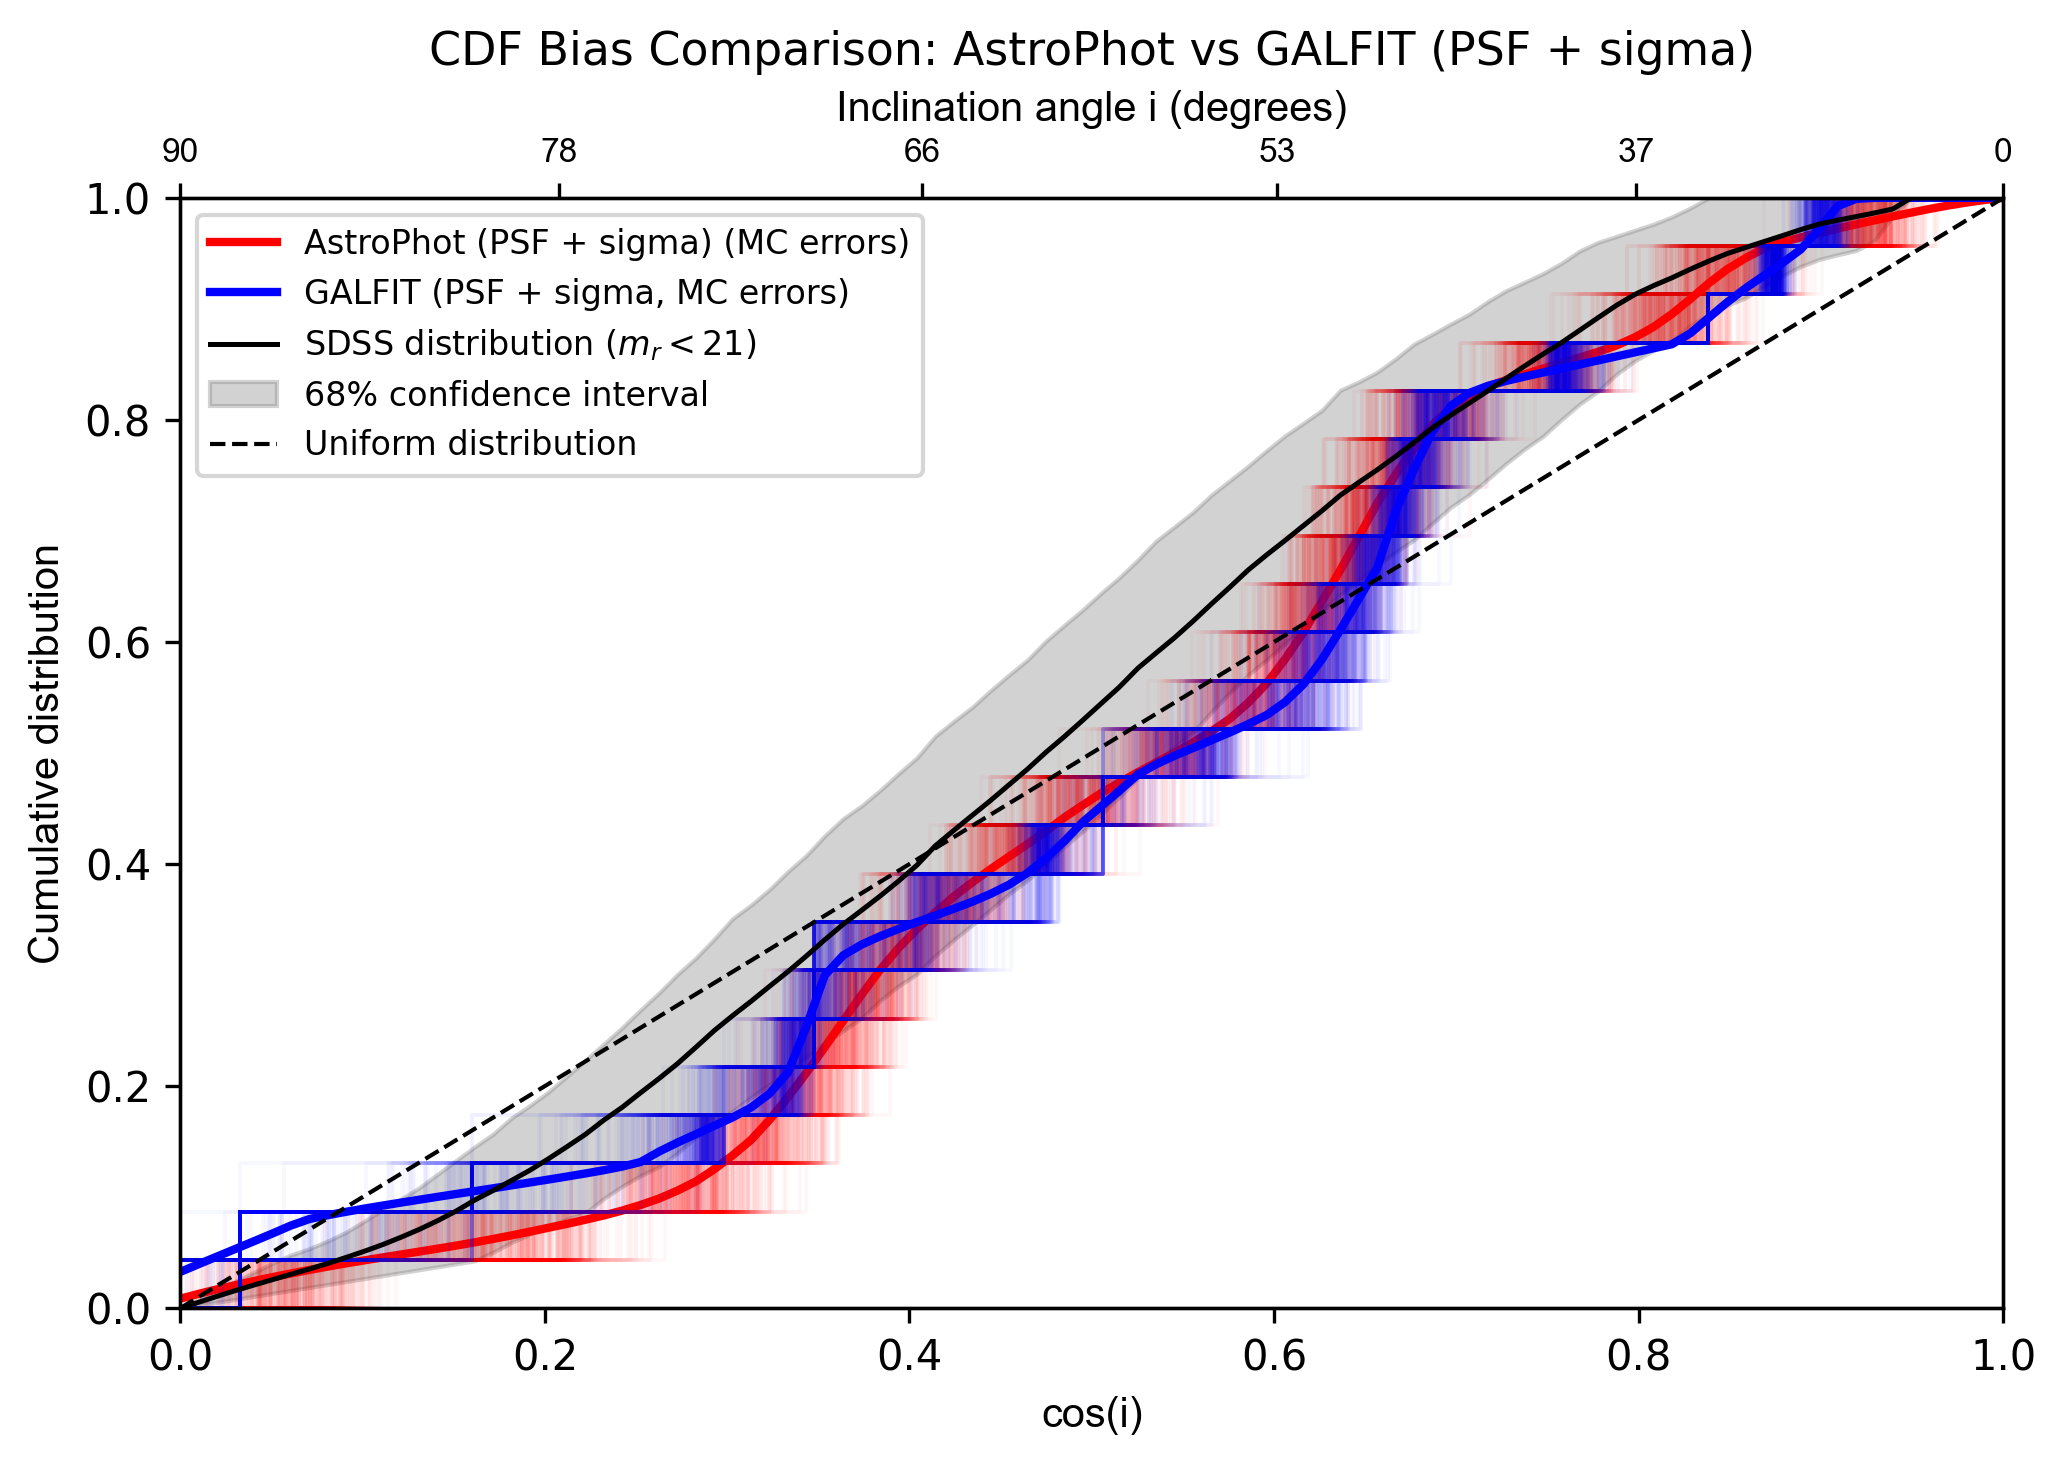
\includegraphics[width=0.92\linewidth]{../../plots/plots_astrophot_psf_sigma/CDF_bias_comparison_psf_sigma_updated_mc_both.png}
    \caption{GALFIT versus AstroPhot comparison where both methods are shown with Monte Carlo uncertainty draws.}
\end{figure}

\section{GALFIT Inclination Angles}
\begin{longtable}{lrrrr}
\caption{GALFIT PSF+sigma inclination angles with propagated uncertainties.}\label{tab:galfit_inclinations} \\
\hline
 FRB & $b/a$ & $\sigma_{b/a}$ & $i_{\mathrm{GALFIT}}$ [deg] & $\sigma_i$ [deg] \\
\hline
\endfirsthead
\hline
 FRB & $b/a$ & $\sigma_{b/a}$ & $i_{\mathrm{GALFIT}}$ [deg] & $\sigma_i$ [deg] \\
\hline
\endhead
 20171020A & 0.390 & 0.000 & 70.02 & 0.00 \\
 20180924B & 0.650 & 0.010 & 50.86 & 0.80 \\
 20190102C & 0.400 & 0.030 & 69.30 & 2.18 \\
 20190608B & 0.680 & 0.000 & 48.45 & 0.00 \\
 20190714A & 0.380 & 0.010 & 70.75 & 0.73 \\
 20191001A & 0.520 & 0.000 & 60.67 & 0.00 \\
 20200906A & 0.320 & 0.000 & 75.23 & 0.00 \\
 20210320C & 0.700 & 0.020 & 46.79 & 1.70 \\
 20210410D & 0.140 & 0.090 & 90.00 & 6.66 \\
 20210807D & 0.700 & 0.010 & 46.79 & 0.84 \\
 20211127I & 0.910 & 0.010 & 25.03 & 1.46 \\
 20211203C & 0.420 & 0.080 & 67.86 & 5.85 \\
 20211212A & 0.830 & 0.000 & 34.70 & 0.00 \\
 20220207C & 0.210 & 0.000 & 86.25 & 0.00 \\
 20220307B & 0.650 & 0.030 & 50.86 & 2.41 \\
 20220310F & 0.690 & 0.020 & 47.62 & 1.67 \\
 20220319D & 0.900 & 0.010 & 26.42 & 1.38 \\
 20220509G & 0.400 & 0.000 & 69.30 & 0.00 \\
 20220825A & 0.630 & 0.050 & 52.43 & 3.98 \\
 20220912A & 0.640 & 0.030 & 51.65 & 2.39 \\
 20220914A & 0.490 & 0.010 & 62.84 & 0.72 \\
 20220920A & 0.860 & 0.000 & 31.39 & 0.00 \\
 20221012A & 0.550 & 0.000 & 58.47 & 0.00 \\
\hline
\end{longtable}

\section{Legacy Survey Inclinations vs GALFIT}
Legacy/Tractor fields queried for host matching and shape-based inclination were \texttt{objid}, \texttt{ra}, \texttt{dec}, \texttt{type}, \texttt{flux\_r}, \texttt{sersic}, \texttt{shape\_e1}, and \texttt{shape\_e2}.
Legacy inclination was derived from shape terms as $|e|=\sqrt{e_1^2+e_2^2}$, $q=(1-|e|)/(1+|e|)$, and $i=\cos^{-1}\!\left(\sqrt{(q^2-q_0^2)/(1-q_0^2)}\right)$ with $q_0=0.2$.
A direct TAP schema query found \texttt{shape\_e1\_ivar} and \texttt{shape\_e2\_ivar}; we convert ivar to standard deviation with $\sigma=1/\sqrt{\mathrm{ivar}}$ and propagate to $\sigma_{i,\mathrm{LS}}$ using Monte Carlo draws in $(e_1,e_2)$ space.
\small
\setlength{\tabcolsep}{4pt}
\renewcommand{\arraystretch}{1.08}
\begin{longtable}{llrrrrrr}
\caption{Legacy Survey inclination angles versus GALFIT inclinations, with Legacy inclination uncertainty propagated from Tractor shape ivars.}\label{tab:legacy_vs_galfit} \\
\hline
 FRB & Type & $n_{LS}$ & $i_{LS}$ & $\sigma_{i,LS}$ & $i_{GF}$ & $\sigma_{i,GF}$ & $\Delta i$ \\
\hline
\endfirsthead
\hline
 FRB & Type & $n_{LS}$ & $i_{LS}$ & $\sigma_{i,LS}$ & $i_{GF}$ & $\sigma_{i,GF}$ & $\Delta i$ \\
\hline
\endhead
 20180924B & SER & 3.32 & 48.12 & 0.43 & 33.63 & 0.80 & 14.49 \\
 20190102C & SER & 0.50 & 64.71 & 1.32 & 80.24 & 2.18 & -15.53 \\
 20190608B & SER & 3.49 & 54.32 & 0.11 & 32.52 & 0.00 & 21.80 \\
 20190714A & SER & 0.53 & 68.70 & 0.38 & 70.75 & 0.73 & -2.05 \\
 20191001A & SER & 0.50 & 82.06 & 2.31 & 46.79 & 0.00 & 35.27 \\
 20200906A & SER & 0.75 & 74.90 & 0.23 & 77.62 & 0.00 & -2.72 \\
 20210320C & REX & -- & 0.00 & -- & 45.10 & 1.70 & -45.10 \\
 20210410D & EXP & -- & 74.99 & 1.78 & 90.00 & 6.66 & -15.01 \\
 20211203C & EXP & -- & 62.89 & 4.09 & 56.24 & 5.85 & 6.65 \\
 20211212A & SER & 1.14 & 35.08 & 0.04 & 32.52 & 0.00 & 2.56 \\
 20220310F & EXP & -- & 49.87 & 2.32 & 70.02 & 1.67 & -20.15 \\
 20220509G & SER & 2.47 & 59.35 & 0.07 & 62.11 & 0.00 & -2.76 \\
 20220914A & SER & 2.03 & 63.08 & 0.70 & 59.94 & 0.72 & 3.14 \\
 20220920A & REX & -- & 0.00 & -- & 31.39 & 0.00 & -31.39 \\
 20221012A & SER & 2.27 & 59.53 & 0.34 & 59.21 & 0.00 & 0.32 \\
\hline
\end{longtable}
\renewcommand{\arraystretch}{1.0}
\normalsize

\end{document}
